\documentclass[
ngerman,
twoside,
pdfa=false,
ruledheaders=section,%Ebene bis zu der die Überschriften mit Linien abgetrennt werden, vgl. DEMO-TUDaPub
class=report,% Basisdokumentenklasse. Wählt die Korrespondierende KOMA-Script Klasse
thesis={type=sta},% Dokumententyp Thesis, für Dissertationen siehe die Demo-Datei DEMO-TUDaPhd
accentcolor=TUDa-2c,% Auswahl der Akzentfarbe
custommargins=false,% Ränder werden mithilfe von typearea automatisch berechnet
marginpar=false,% Kopfzeile und Fußzeile erstrecken sich nicht über die Randnotizspalte
%BCOR=5mm,%Bindekorrektur, falls notwendig
parskip=half-,%Absatzkennzeichnung durch Abstand vgl. KOMA-Sript
fontsize=11pt,%Basisschriftgröße laut Corporate Design ist mit 9pt häufig zu klein
%	logofile=tuda_logo.pdf, %Falls die Logo Dateien nicht installiert sind
]{tudapub}

%%%%%%%%%%%%%%%%%%%%%%%%%%%%
% Download des TU-Logos
%%%%%%%%%%%%%%%%%%%%%%%%%%%%
% https://download.hrz.tu-darmstadt.de/protected/CE/TUDa_LaTeX/tuda_logo.pdf
% Der Pfad zum Logo kann als "logofile" angegeben werden.

%%%%%%%%%%%%%%%%%%%
% Sprachanpassung & Verbesserte Trennregeln
%%%%%%%%%%%%%%%%%%%
\usepackage[english, main=ngerman]{babel}
\usepackage[autostyle]{csquotes}% Anführungszeichen vereinfacht
\usepackage{microtype}

%%%%%%%%%%%%%%%%%%%
% Literaturverzeichnis
%%%%%%%%%%%%%%%%%%%
\usepackage{biblatex}   % Literaturverzeichnis
\addbibresource{HausarbeitBib.bib}

%%%%%%%%%%%%%%%%%%%
% Paketvorschläge Tabellen
%%%%%%%%%%%%%%%%%%%
%\usepackage{array}     % Basispaket für Tabellenkonfiguration, wird von den folgenden automatisch geladen
\usepackage{tabularx}   % Tabellen, die sich automatisch der Breite anpassen
%\usepackage{longtable} % Mehrseitige Tabellen
%\usepackage{xltabular} % Mehrseitige Tabellen mit anpassarer Breite
\usepackage{booktabs}   % Verbesserte Möglichkeiten für Tabellenlayout über horizontale Linien

%%%%%%%%%%%%%%%%%%%
% Paketvorschläge Mathematik
%%%%%%%%%%%%%%%%%%%
\usepackage{mathtools} % erweiterte Fassung von amsmath
\usepackage{amssymb}   % erweiterter Zeichensatz
\usepackage[decimalsymbol=comma]{siunitx}   % Einheiten
\usepackage{amsmath}


%%%%%%%%%%%%%%%%%
% Eigenen Pakete Gruppe03
%%%%%%%%%%%%%%%%%%%%
%\usepackage[utf8]{inputenc}
%\usepackage[ngerman]{babel}
\usepackage{hyperref}
\usepackage{graphicx}
\usepackage{subcaption}
\usepackage{listings}
\usepackage[framed, numbered]{matlab-prettifier}
%\usepackage[style=numeric]{biblatex}
%\usepackage{amsthm}
%\usepackage[squaren]{SIunits}
\usepackage{enumitem}
\usepackage{tikz}
\usepackage{pgfplots}
\usepackage{pgfplotstable}
%\usepackage{booktabs}
\pgfplotsset{compat=1.12}
\usepackage{dsfont}

%%%%%%%%%%%%%%%%%%%
% verschiedene Nummerierung für Abbildungen und Formeln
%%%%%%%%%%%%%%%%%%%
\usepackage{chngcntr}
\counterwithout{equation}{chapter}


%%%%%%%%%%%%%%%%%%%
% Pseudocode
%%%%%%%%%%%%%%%%%%%
\usepackage[linesnumbered,lined,boxruled]{algorithm2e} % Package für Pseudocode

%%%%%%%%%%%%%%%%%%%
% Plotting und Grafik
%%%%%%%%%%%%%%%%%%%
\usepackage{tuda-pgfplots} % Package für Plotting with TUDa mods

%%%%%%%%%%%%%%%%%%%
% Sonstiges
%%%%%%%%%%%%%%%%%%%
\usepackage{blindtext} % Package für Blindtext

\begin{document}
	\title{Ausarbeitung Übung 3}
	%\subtitle{Ein Untertitel, wenn nötig}
	\author[D. Schiller, C. Kramer, S.Arnold, T. Lingenberg]{Dominik Schiller \and Constanze Kramer \and Simon Arnold \and Tobias Lingenberg} %optionales Argument ist die Signatur,
	%\reviewer{Gutachter 1 \and Gutachterin 2} %Gutachten
	
	%Diese Felder werden untereinander auf der Titelseite platziert.
	\department{} % Das Kürzel wird automatisch ersetzt und als Studienfach gewählt, siehe Liste der Kürzel im Dokument.

	
	\date{\today}
	%\examdate{\today}
	
	%	\tuprints{urn=1234,printid=12345}
	%	\dedication{Für alle, die \TeX{} nutzen.}
	
	\maketitle
	\pagenumbering{gobble} % Seitenzahlen angezeigt, startet ab dem Inhaltsverzeichnis
	
	
	%\affidavit
	%\AffidavitSignature
	%\AffidavitSignature
	
	
	%%%%%%%%%%%%%%%%%%%
	%Abstract / Kurzzusammenfassung
	%%%%%%%%%%%%%%%%%%%
	%\include{chapters/zusammenfassung}
	
	%%%%%%%%%%%%%%%%%%%
	%Inhaltsverzeichnis 
	%%%%%%%%%%%%%%%%%%%
	\cleardoublepage
	\tableofcontents % Erstellte ein Inhaltsverzeichnis
	
	%\cleardoublepage
	\pagenumbering{arabic} % Seitenzahlen angezeigt, startet ab dem Inhaltsverzeichnis
	\setcounter{page}{1} % Setzt den Seitenzahlenzähler auf 1
	\chapter{Einleitung}\label{sec:intro}
Diese Arbeit beschäftigt sich mit dem Übungsblatt 9 des Faches \glqq Einführung in die numerische Berechnung elektromagnetischer Felder\grqq{}.
Zunächst wird der primale Divergenz und Rotationsoperator in Octave implementiert und berechnet. Anschließend wird eine Materialmatrix berechnet. Abschließend wird das Magnetfeld von zwei stromdruchflossenen Leitern in Octave simuliert. 
	%%%%%%%%%%%%%%%%%%%%%%%%%%%%%%%%%%%%%%%%%%%%%%%%%%%%%%%%%%%%%%%%%%%%%%%%%%%%%%%%%%%%%%%%%%%%%%%%%%
	
	% INHALT, am Besten ausgelagert in eigene Files/Kapitel und dann mit \include{Unterordner/Filename} eingefügt, sorgt für bessere Übersichtlichkeit und Fehlersuche. Einzelne Dateien sind aktuell im Ordner Sections abgelegt. 
	%%%%%%%%%%%%%%%%%%Einleitung%%%%%%%%%%%%%%%%%
	
	%%%%%%%%%%%%%%%%%%Haupteil%%%%%%%%%%%%%%%%%%%
	\section{Koaxialkabel Simulator}\label{sec:ag3_1}

Das elektrische Verhalten eines Koaxialkabels lässt sich durch das Ersatzschaltbild \ref{koaxialkabel1} beschreiben. Hierbei stellt $R_1$ den ohmschen Längswiderstand dar, der von der Leitungslänge, dem Leitungsquerschnitt und dem Material abhängt.

Das induktive Verhalten des Kabels wird durch $L_1$ simuliert. Jeder stromdurchflossene Leiter baut ein Magnetfeld auf, die Änderung des Magnetfelds induziert eine Spannung, die dem Stromfluss entgegen wirkt und diesen abschwächt.

Durch den Isolationswert $R_2$ werden Verlustströme betrachtet, die zwischen dem inneren und äußeren Leiter des Koaxialkabels auftreten. Diese Leckströme entstehen, da es in der Realität keinen idealen Isolator gibt.

Zuletzt beinhaltet das Ersatzschaltbild noch die Leitungskapazität $C_1$. Ist am Ende der Leitung ein Verbraucher $R_f$ angeschlossen, so liegt an diesem eine Spannung an. In Folge dessen besteht auch zwischen Hin- und Rückleiter eine Potenzialgefälle. Beide Leiter verhalten sich, aufgrund der Ladungsdifferenz, somit wie die Platten eines Kondensators\footnote{Quelle: Leitungstechnik, Dipl.-Ing.(FH) Christian Wolff, 2009}. 

\begin{figure}[h]
	\centering
	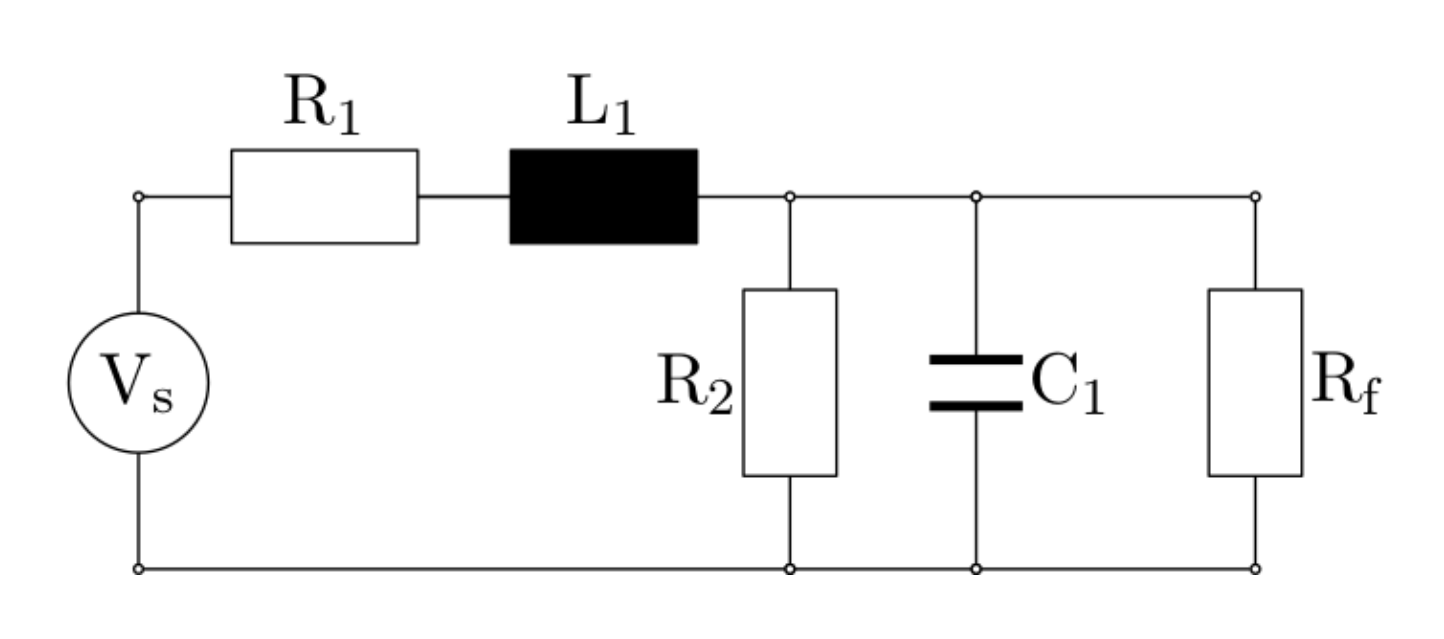
\includegraphics[width=0.7\textwidth]{data/Koaxialkabel1}
	\caption{Ersatzschaltbild Koaxialkabel}
	\label{koaxialkabel1}
\end{figure}

Mit den Routinen, die in Aufgabe 2.3 entwickelt wurden lässt sich nun dieses Segment eines Koaxialkabels simulieren. Hierzu übergibt man der Methode \texttt{calculate\_matrices} (siehe \ref{calculate_matrices}) die Netzliste \ref{netlist1}.

\begin{lstlisting}[caption={Netzliste Koaxialkabel}, label=netlist1]
Vs 1 0 12
L1 2 3 0.00025
R1 1 2 0.001
C1 3 0 0.0000001
R2 0 3 1500
Rf 0 3 1500
\end{lstlisting}

\newpage
Berechnet werden nun wieder die Matrizen $\mathbf{M, K}$ und $\mathbf{r}$, die die Differenzialgleichung
\begin{equation}
\mathbf{M} \frac{\text{d}}{\text{d}t} \mathbf{x} + \mathbf{K} \mathbf{x} = \mathbf{r}
\label{matrixDGL}
\end{equation}

parametrisieren. Zuletzt wird mit der Funktion \texttt{daspk} das Gleichungssystem numerisch gelöst und die Spannung an $R_f$ gezeichnet \ref{plottKK1}. Das dazu verwendete Skript befindet sich im Anhang \ref{finalesSkript}.

\begin{figure}[h]
	\centering
	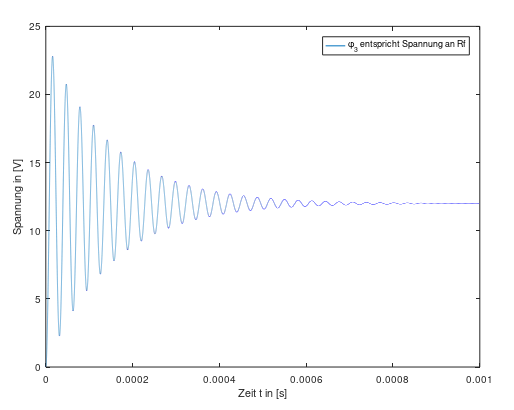
\includegraphics[width=0.7\textwidth]{data/plotKK1}
	\caption{Spannungsverlauf an Last $R_f$ bei konstanter Spannungsquelle mit 12\si{\volt}}
	\label{plottKK1}
\end{figure}

\subsubsection{Koaxialkabel mit n Gliedern}
Nun wird das RLC-Segment in \ref{koaxialkabel1} $n=10$ mal hintereinander in Reihe geschaltet (siehe \ref{koaxialkabel10}).

\begin{figure}[h]
	\centering
	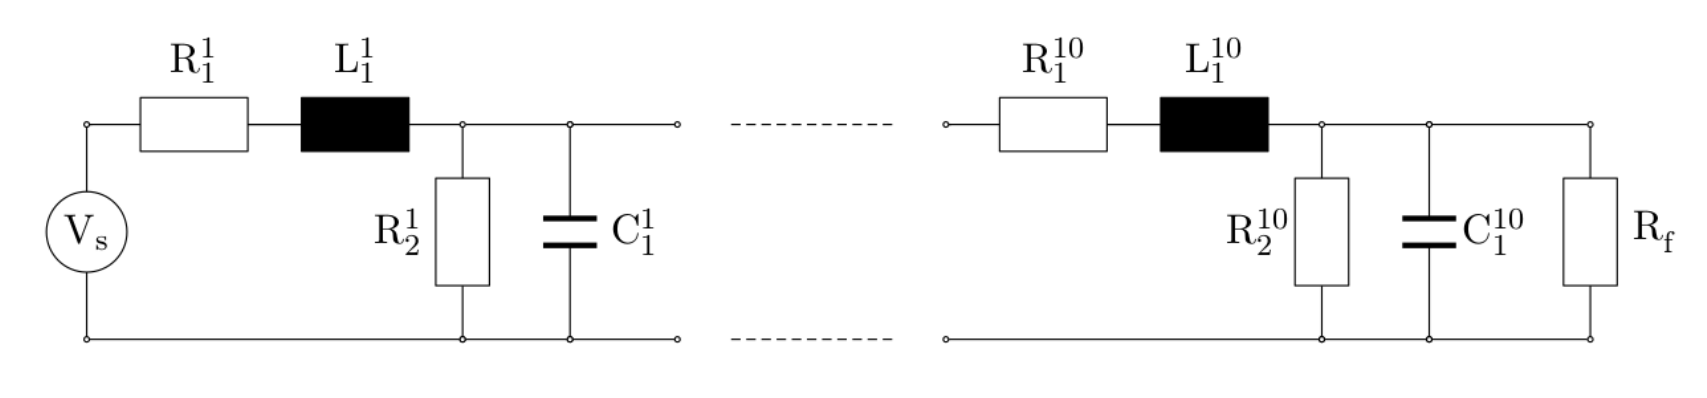
\includegraphics[width= 0.9\textwidth]{data/Koaxialkabel10}
	\caption{Ersatzschaltbild Koaxialkabel mit $n=10$ Segmenten}
	\label{koaxialkabel10}
\end{figure}

\newpage
Um zu untersuchen inwiefern diese Veränderung auf die Spannung an $R_f$ Einfluss hat, wurde ein neues Skript geschrieben, das die Unterschiede der Ausgangsspannung bei $n=1$ und $n=10$ sichtbar macht (siehe \ref{finalesSkript10}). Hierzu wurde die Netzliste für $n=10$ Segmente erstellt (siehe \ref{netlist10}), den Methoden übergeben und die Spannung an $R_f$ erneut berechnet.
Beide Ausgangsspannungen für $n=1$ und $n=10$ wurden nun in das selbe Diagramm \ref{plottKK10} eingezeichnet:

\begin{figure}[h]
	\centering
	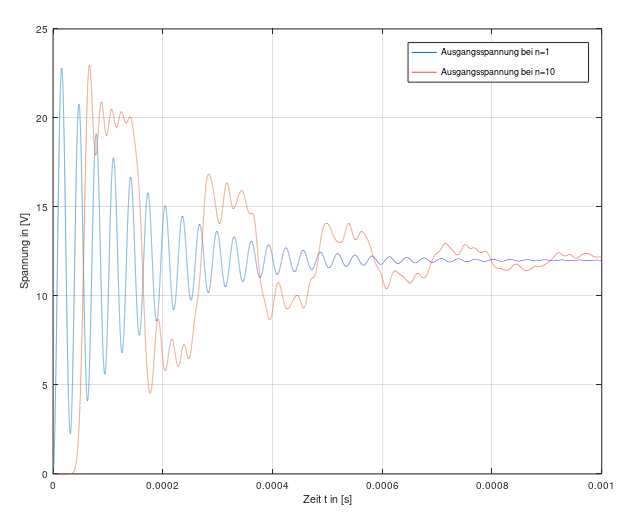
\includegraphics[width=0.75\textwidth]{data/plotKK10}
	\caption{Spannungsverlauf an Last $R_f$ für $n=1$ und $n=10$}
	\label{plottKK10}
\end{figure}

Auffällig ist zunächst einmal, dass im Fall $n=10$ das Signal durch Oberschwingungen gestört wird. Jedoch lässt sich die eigentliche Hauptschwingung dennoch gut erkennen. Bei Betrachtung dieser im Vergleich zum Fall $n=1$ wird ebenso deutlich, dass die Frequenz erheblich verzögert wurde. Ein weiterer Unterschied besteht in der Dämpfung, welche bei n=10 nicht so stark ist . Es dauert länger, bis die Amplitude gegen $0$ geht. Zuletzt ist noch anzumerken, dass der maximal Betrag der Spannung an $R_f$ in beiden Fällen gleich ist. Die Spannung liegt immer zwischen $0$ und $24\si{\volt}$.

Empirische Tests ergaben, dass diese Aussagen für alle $n>1, n \in \mathbb{N}$ gelten. Folglich gilt, je mehr Segmente hinzugefügt werden, umso mehr verzögert sich die Frequenz. Der maximale Betrag der Spannung an der Last hängt jedoch nicht von $n$ ab. Der erste Ausschlag erreicht jedes mal das maximale Niveau von knapp unter $24\si{\volt}$ und nimmt dann mit der Zeit immer weiter ab, bis die Spannung gegen $12\si{\volt}$ konvergiert.
	\section{Frequenzbereich}\label{sec:ag3_2}
<<<<<<< HEAD
a)
\begin{gather*}
\alpha(t)=-kx(t)+cos(\omega t)\\
x(t)=e{^-k(t-t_0)}(x_0)+\int_{t_0}^{t} e^{k(s-t_0)}cos(\omega s)ds\\
f'=e^{k(s-t_0)}\\
g=cos(\omega s)\\
\end{gather*}
partiell integrieren
\begin{gather*}
f=\frac{e^{k(s-t_0)}}{k}\\
g'=-\omega sind(\omega s)\\
(e^{-k(t-t_0)}x_0)+[\frac{e^{k(t-t_0)}cos(\omega s)}{k}]^{s=t}_{s=t_0}-\int_{t_0}^{t}-\frac{\omega sin(\omega s)e^{k(s-t_0)}}{k}ds\\
\end{gather*}
partiell integrieren
\begin{gather*}
f'=\frac{e^{k(s-t_0)}}{k}\\
g=-\omega sin(\omega s)\\
f=\frac{e^{k(s-t_0)}}{k^2}\\
g'=-\omega^2 sin(\omega s)\\
\end{gather*}
\begin{gather*}
(e^{-k(t-t_0)}x_0)+[\frac{e^{k(t-t_0)}cos(\omega s)}{k}]^{t}_{s=t_0}-(-[\frac{\omega^{k(s-t_0)}sin(\omega s)}{k^2}]^{t}_{s=t_0}\int_{t_0}^{t}-\frac{\omega^2 e^{k(s-t_0)}cos(\omega s)}{k^2}ds)\\
(e^{-k(t-t_0)}x_0)+\int_{t_0}^{t}e^{k(s-t_0)}cos(\omega s)ds=[\frac{e^{k(t-t_0)}cos(\omega s)}{k}]^{t}_{s=t_0}+[\frac{\omega^{k(s-t_0)}sin(\omega s)}{k^2}]^{t}_{s=t_0}-\frac{\omega^2}{h^2}\int_{t}^{s=t_0}e^{k(s-t_0)}cos(\omega s)ds\\
\int_{t_0}^{t}e^{k(s-t_0)}cos(\omega s)ds+\frac{\omega^2}{k^2}\int_{t}^{t_0}e^{k(s-t_0)}cos(\omega s)ds=[\frac{e^{k(s-t_0)}cos(\omega s)}{k}]^{t}_{s=t_0}+[\frac{\omega e^{k(s-t_0)}sin(\omega s)}{k^2}]^{t}_{s=t_0}\\
\int_{t_0}^{t}e^{k(s-t_0)}cos(\omega s)ds+(1+\frac{\omega^2}{h^2})=[\frac{e^{k(t-t_0)}cos(\omega s)}{k}]^{t}_{s=t_0}+[\frac{\omega e^{k(s-t_0)}sin(\omega s)}{k^2}]^{t}_{s=t_0}\\
\int_{t_0}^{t}e^{k(s-t_0)}cos(\omega s)ds+(\frac{k^2+\omega^2}{h^2})=[\frac{e^{k(t-t_0)}cos(\omega s)}{k}]^{t}_{s=t_0}+[\frac{\omega e^{k(s-t_0)}sin(\omega s)}{k^2}]^{t}_{s=t_0}\\
\int_{t_0}^{t}e^{k(s-t_0)}cos(\omega s)ds=([\frac{e^{k(t-t_0)}cos(\omega s)}{k}]^{t}_{s=t_0}+[\frac{\omega e^{k(s-t_0)}sin(\omega s)}{k^2}]^{t}_{s=t_0})*(\frac{k^2+\omega^2}{h^2})\\
=[\frac{ke^{k(t-t_0)}cos(\omega s)+\omega e^{k(s-t_0)}sin(\omega s)}{\omega^2+k^2}]^{t}_{s=t_0}\\
=\frac{[e^{k(t-t_0)}cos(\omega s)+\omega e^{k(s-t_0)}sin(\omega s)]^{t}_{s=t_0}}{\omega^2+k^2}\\
e^{-kt+kt_0}=\frac{e^{kt_0}}{e^{kt}}\\
=\frac{\omega e^{kt}sin(\omega t)+ke^{kt}cos(\omega t)}{e^{kt_0}(\omega^2+k^2)}-\frac{\omega sin(\omega t_0)+kcos(\omega t_0)}{(\omega^2+k^2)}\\
x(t)=e^{-k(t-t_0)}(x_0+\frac{\omega e^{kt}sin(\omega t)+ke^{kt}cos(\omega t)}{e^{kt_0}(\omega^2+k^2)}-\frac{\omega sin(\omega t_0)+kcos(\omega t_0)}{(\omega^2+k^2)})\\
=\frac{\omega sin(\omega t)+kcos(\omega t)}{(\omega^2+k^2)}-e^{-k(t-t_0)}(\frac{\omega sin(\omega t_0)+kcos(\omega t_0)}{(\omega^2+k^2)}-x_0)\\
=e^{-k(t-7_0)}(x_0-\frac{\omega sin(\omega t_0)+kcos(\omega t_0)}{(\omega^2+k^2)})+\frac{\omega sin(\omega t)+kcos(\omega t)}{(\omega^2+k^2)}
\end{gather*}
b)
\begin{gather*}
x_{freq} (t)=Re\{\underline{\alpha} e^{j\omega t}\}\\
x'_{freq} (t)=Re\{j \omega \underline{x} e^{j\omega t}\}\\
Re\{j \omega \underline{x} e^{j\omega t}\}=-kRe\{\underline{x} e^{j\omega t}\}-Re\{ e^{j\omega t}\}\\
Re\{j \omega \underline{x} e^{j\omega t}\}+kRe\{\underline{x} e^{j\omega t}\}+Re\{ e^{j\omega t}\}=0\\
Re\{(j\omega \underline{x}+k\underline{x}-1)e^{j\omega t}\}=0\\
j\omega\underline{x}+k\underline{x}=1=0\\
\underline{x}=\frac{1}{k+j\omega}=\frac{k-j\omega}{k^2+\omega^2}\\
(e^{j\omega t}=cos(\omega t)+j sin(\omega t))\\
\Downarrow\\
x_{freq}(t)=Re\{\frac{k-j\omega}{k^2+\omega^2}(cos(\omega t)+jsin(\omega t))\}\\
=\frac{kcos(\omega t)+\omega sin(\omega t)}{k^2+\omega^2}
\end{gather*}
=======

In der Elektrotechnik arbeitet man oft an Problemen mit sinus-förmigen Schwingungen. Um die Rechnungen dafür zu vereinfachen bietet es sich an diese Probleme nur im Frequenzbereich zu betrachten. 
Im folgenden wird allerdings zuerst eine Lösung für die skalare lineare gewöhnliche Differentialgleichung im Zeitbereich 

\begin{equation}
	x'(t) = f(t,x) := -kx(t) +r(t)
	\label{DGL}
\end{equation}

mit Startwert $x(t_0) = x_0$ und $k > 0$ ermittelt. Die Anregung ist durch $r(t) = \mathrm{cos}(\omega t)$ als sinus-förmige Schwingung gegeben, wobei $\omega$ die Kreisfrequenz ist.
Aus der vorgegebenen allgemeinen Lösung 

\begin{equation}
	x(t)=\mathrm{e}^{-k(t-t_0)} \left(x_0+\int_{t_0}^{t} \mathrm{e}^{k(s-t_0)}r(s)ds\right)
	\label{Ansatz}
\end{equation} 

betrachtet man vorerst nur das Integral und löst dieses.\\
Für die partielle Integrationsregel 

\begin{equation*}
	\int_{a}^{b}f'(x) \cdot g(x)dx = \left[f(x) \cdot g(x)\right]^{b}_{a} - \int_{a}^{b} f(x) \cdot g'(x)dx
\end{equation*}

setzt man nun $f'(x)=\mathrm{e}^{k(s-t_0)}$ und $g(x)=\mathrm{cos}(\omega s)$. Daraus ergibt sich $f(x)=\frac{1}{k}\mathrm{e}^{k(s-t_0)}$ sowie $g'(x)=-\omega \mathrm{sin}(\omega s)$. Eingesetzt ergibt dies 

\begin{equation*}
	\int_{t_0}^{t} \mathrm{e}^{k(s-t_0)}\mathrm{cos}(\omega s)ds = \left[ \frac{\mathrm{e}^{k(s-t_0)}\mathrm{cos}(\omega s)}{k} \right]^{t}_{s=t_0}-\int_{t_0}^{t}-\frac{\omega \mathrm{sin}(\omega s)\mathrm{e}^{k(s-t_0)}}{k} ds.
\end{equation*}

Unter der Annahme $f'(x)=\frac{\mathrm{e}^{k(s-t_0)}}{k}$, $g(x)=-\omega \mathrm{sin}(\omega s)$ wird erneut partiell integriert, damit folgt $f(x)=\frac{\mathrm{e}^{k(s-t_0)}}{k^2}$ und $g'(x)=-\omega^2 \mathrm{sin}(\omega s)$. Setzt man die Annahmen in die vorherige Gleichung ein, folgt

\begin{equation*}
	\int_{t_0}^{t} \mathrm{e}^{k(s-t_0)}\mathrm{cos}(\omega s)ds = \left[\frac{\mathrm{e}^{k(s-t_0)} \mathrm{cos}(\omega s)}{k}\right]^{t}_{s=t_0}-\left(-\left[\frac{\omega \mathrm{e}^{k(s-t_0)}\mathrm{sin}(\omega s)}{k^2}\right]^{t}_{s=t_0}-\int_{t_0}^{t}-\frac{\omega^2 \mathrm{e}^{k(s-t_0)}\mathrm{cos}(\omega s)}{k^2}ds\right)
\end{equation*} 

dies weiter vereinfacht führt zu 

\begin{equation*}
	\int_{t_0}^{t}\mathrm{e}^{k(s-t_0)}\mathrm{cos}(\omega s)ds = \left[\frac{\mathrm{e}^{k(s-t_0)} \mathrm{cos}(\omega s)}{k}\right]^{t}_{s=t_0} +\left[\frac{\omega\mathrm{e}^{k(s-t_0)} \mathrm{sin}(\omega s)}{k^2}\right]^{t}_{s=t_0}-\frac{\omega^2}{k^2} \int_{s=t_0}^{t}\mathrm{e}^{k(s-t_0)}\mathrm{cos}(\omega s)ds.
\end{equation*}
	
Das Ausgangsintegral findet sich nun sowohl auf der linken, als auch auf der rechten Seite der Gleichung wieder. Die Formel

\begin{equation*}
	\int_{t_0}^{t}\mathrm{e}^{k(s-t_0)}\mathrm{cos}(\omega s)ds \cdot \left(\frac{k^2+\omega^2}{k^2}\right) = \left[\frac{\mathrm{e}^{k(s-t_0)} \mathrm{cos}(\omega s)}{k}\right]^{t}_{s=t_0}+\left[\frac{\omega \mathrm{e}^{k(s-t_0)} \mathrm{sin}(\omega s)}{k^2}\right]^{t}_{s=t_0}
\end{equation*}

ergibt sich durch das Zusammenfassen der beiden gleichen Integrale auf einer Seite. Dividieren durch $\frac{k^2+\omega^2}{k^2}$ und das einsetzen der Integrationsgrenzen führt zu dem Ergebnis des Integrals 

\begin{equation*}
	\int_{t_0}^{t}\mathrm{e}^{k(s-t_0)}\mathrm{cos}(\omega s)ds = 
	\frac{\omega \mathrm{e}^{kt}\mathrm{sin}(\omega t)+k\mathrm{e}^{kt}\mathrm{cos}(\omega t)}{\mathrm{e}^{kt_0}(\omega^2+k^2)}-\frac{\omega \mathrm{sin}(\omega t_0)+k\mathrm{cos}(\omega t_0)}{\omega^2+k^2}.
\end{equation*}

Somit ist die Lösung für (\ref{Ansatz})

\begin{equation*}
	x(t)=\mathrm{e}^{-k(t-t_0)} \left(x_0+\frac{\omega \mathrm{e}^{kt}\mathrm{sin}(\omega t)+k\mathrm{e}^{kt}\mathrm{cos}(\omega t)}{\mathrm{e}^{kt_0}(\omega^2+k^2)}-\frac{\omega \mathrm{sin}(\omega t_0)+k\mathrm{cos}(\omega t_0)}{\omega^2+k^2}\right),
\end{equation*}

durch das Ausmultiplizieren und Aufteilen in den gedämpften Anteil abhängig vom Startwert $x_0$ sowie sinus-förmige Schwingung, erfüllt

\begin{equation}
	x(t) = \mathrm{e}^{-k(t-t_0)}\left(x_0-\frac{\omega \mathrm{sin}(\omega t_0)+k\mathrm{cos}(\omega t_0)}{\omega^2+k^2}\right)+\frac{\omega \mathrm{sin}(\omega t)+k\mathrm{cos}(\omega t)}{\omega^2+k^2}.
	\label{allgemeineLösung}
\end{equation}

die Differentialgleichung (\ref{DGL}) im Zeitbereich.\\

Nach Berechnung der Differentialgleichung im Zeitbereich folgt nun die Betrachtung im Frequenzbereich. Hierbei wird die Lösung als Kosinus unbekannter Amplitude

\begin{equation*}
	x_{freq} (t) = \Re \left\{\underline{x}\mathrm{e}^{j\omega t}\right\}
\end{equation*}

angenommen, mit $\mathrm{cos}(\omega t) = \Re\left\{\mathrm{e}^{j\omega t}\right\}$ wobei $\underline{x}$ der Phasor ist. Die zeitliche Ableitung 

\begin{equation*}
	x'_{freq}(t) = \Re \left\{j\omega \underline{x} \mathrm{e}^{j\omega t}\right\}
\end{equation*}

wird in (\ref{DGL}) eingesetzt, dies liefert

\begin{equation*}
	\Re \left\{j\omega \underline{x} \mathrm{e}^{j\omega t}\right\} = -k\Re\left\{\underline{x}\mathrm{e}^{j\omega t}\right\} + \Re\left\{\mathrm{e}^{j\omega t}\right\}.
\end{equation*}

Umstellen und Zusammenfassen der Terme ergeben die Gleichung

\begin{equation*}
	\Re \left\{(j\omega \underline{x} + k\underline{x} - 1)\mathrm{e}^{j\omega t}\right\} = 0,
\end{equation*}

somit muss $j\omega \underline{x} + k\underline{x} - 1 = 0$ gelten. Nach $\underline{x}$ aufgelöst erhält man 

\begin{equation*}
	\underline{x} = \frac{k-j\omega}{k^2+\omega^2}.
\end{equation*}

Zur Berechnung der Lösung 
\begin{equation}
x_{freq} (t) = \frac{k\mathrm{cos}(\omega t) + \omega\mathrm{sin}(\omega t)}{k^2+ \omega^2}.
\label{lsgfreq}
\end{equation}

im Frequenzbereich (\ref{DGL}) setzt man den berechneten Phasor $\underline{x}$ und die von der Eulerschen in die Polare Darstellung umgerechneten Werte $\mathrm{e}^{j\omega t} = \mathrm{cos}(\omega t) + j\mathrm{sin}(\omega t)$ in $x_{freq}$ ein.



Zwar wird mit dem Ansatz der Lösung im Frequenzbereich das transiente Anfangsverhalten vernachlässigt, jedoch ist die Lösung, verglichen mit dem Ansatz zum Ermitteln des Zeitbereichs, deutlich leichter und weniger zeitaufwändig, da man nur einmal eine sehr einfache Ableitung berechnen muss.\\


Zusätzlich wird eine Reihenschaltung aus einer Spule und einem Widerstand betrachtet ()LR-Schaltung). Diese wird in LT-Spice gebaut und simuliert. Bei der gegebenen Datei  \texttt{Beispielschaltung2.asc} handelt es sich um eine AC-Simulation, aus der das Verhalten der Schaltung in Abhängigkeit von verschiedenen Frequenzen, in diesem Fall von $f=\SI{100}{\hertz}$ bis $f=\SI{1}{\mega\hertz}$, abgelesen werden kann. 

\begin{figure}[h]
	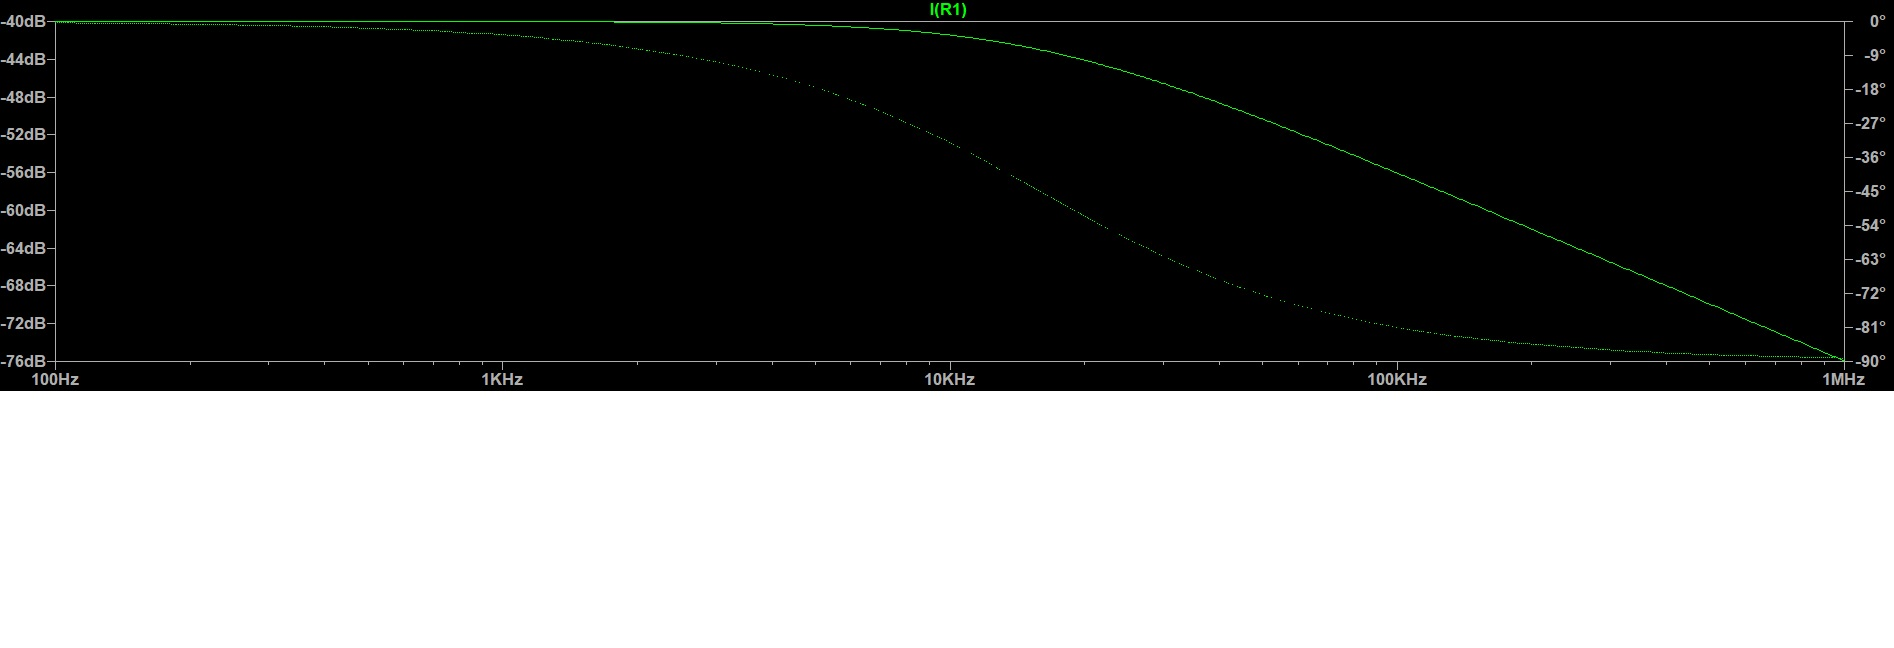
\includegraphics[width=\textwidth]{data/spiceplot32}
	\caption{AC-Simulation aus LT-Spice}
	\label{spiceplot}
\end{figure}

Die Schaltung lässt sich durch die Differentialgleichung

\begin{equation}
	\frac{\mathrm{d}}{\mathrm{d}t}i(t) = -\frac{R}{L}i(t) +\frac{1}{L}u_i(t)
	\label{spezielleDGL}
\end{equation}

beschreiben wobei $R$ der Widerstand, $L$ die Induktivität, $i(t)$ der Strom und $u_i(t)=\mathrm{cos}(\omega t)$ die anregende Spannung ist. Die Lösung für diese Differentialgleichung im Zeitbereich lässt sich mit Hilfe von (\ref{allgemeineLösung}) ermitteln. Hierfür setzt man für $x(t) = i(t)$, $k=\frac{R}{L}$ und für $r(t) = \frac{1}{L}\mathrm{cos}(\omega t)$ ein. Erweitert man im selben Schritt auch noch die Brüche mit $\frac{L}{L}$ so folgt daraus als Lösung für (\ref{spezielleDGL})

\begin{equation*}
	i(t) = \mathrm{e}^{-\frac{R}{L}(t-t_0)}\left(x_0-\frac{L\omega \mathrm{sin}(\omega t_0)+R\mathrm{cos}(\omega t_0)}{L^2\omega^2+k^2}\right)+\frac{L\omega \mathrm{sin}(\omega t)+R\mathrm{cos}(\omega t)}{L^2\omega^2+k^2}.
\end{equation*}

Analog ergibt sich die Lösung im Frequenzbereich durch einsetzen in (\ref{lsgfreq}) mit

\begin{equation*}
	i_{freq} (t) = \frac{R\mathrm{cos}(\omega t) + L\omega\mathrm{sin}(\omega t)}{R^2+ L^2\omega^2}.
\end{equation*}

Die Spannung über dem Widerstand lautet dann nach dem Ohm'schen Gesetz $U=R\cdot I$ und mit der Frequenz $f=\frac{\omega}{2\pi}$

\begin{equation*}
u_{R} (t) = \frac{R\mathrm{cos}(2\pi ft) + 2\pi fL\mathrm{sin}(2\pi ft)}{R^2+ (2\pi fL)^2}R.
\end{equation*}

Das Schaubild für diese Funktion sieht man in Abbildung \ref{spannungplot}.

\begin{figure}[h]
	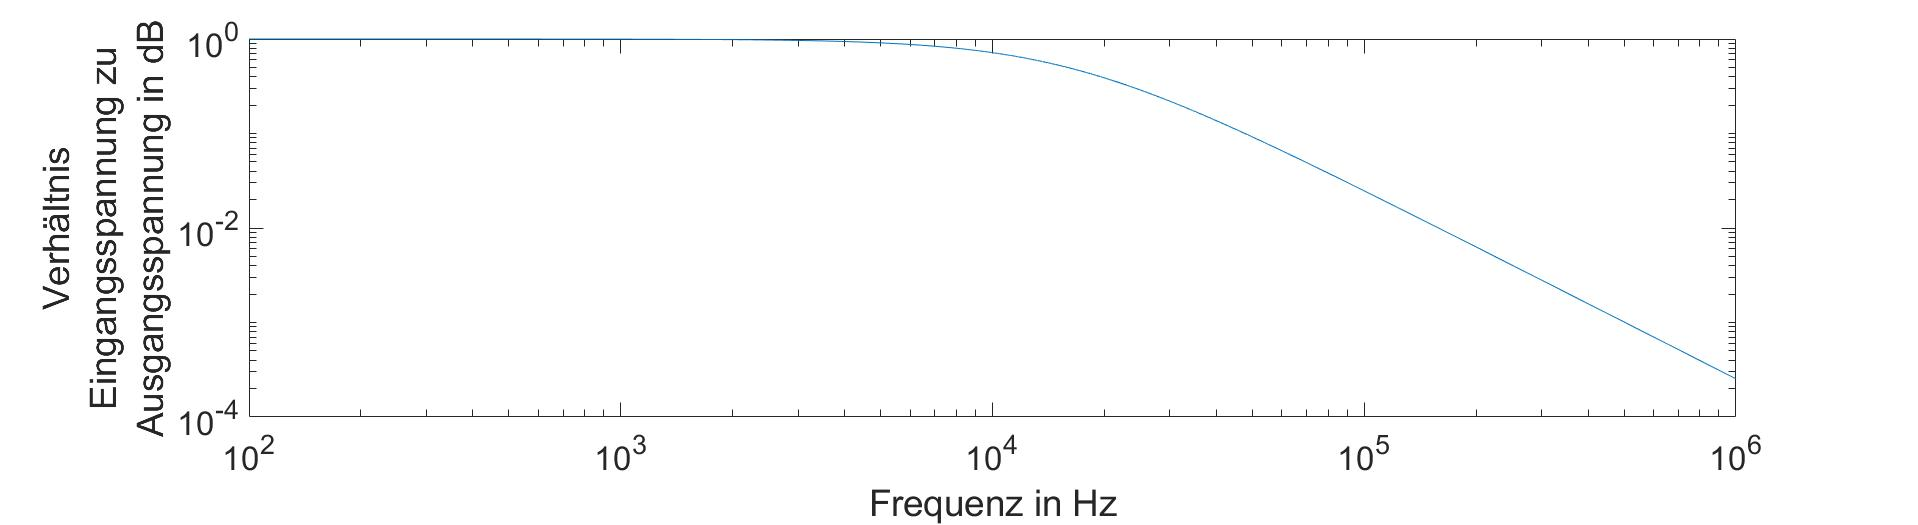
\includegraphics[width=\textwidth]{data/nocheinversuch.jpg}
	\caption{MATLAB-Plot der Spannung über dem Widerstand R}
	\label{spannungplot}
\end{figure}

Anhand des Frequenzgangs fällt auf, dass es sich um eine Schaltung mit Tiefpass-Verhalten handelt, denn bei niedrigen Frequenzen bis ca. $\SI{10}{\kilo\hertz}$ ist die Ausgangsspannung genauso groß wie die Eingangsspannung. Bei hohen Frequenzen nahe $\SI{1}{\mega \hertz}$ ist die Ausgangsspannung deutlich geringer als die Eingangsspannung.




>>>>>>> main

	\section{Simulation homogener Plattenkondensator}\label{sec:ag3_3}
In dieser Aufgabe wird ein harmonischer Plattenkondensator in dem Simulationsprogramm \glqq FEMM \grqq{} nachgebaut. FEMM steht kostenfrei zur Verfügung und kann in Octave eingebunden werden.\\
Zunächst soll der Einfluss unterschiedlicher Randbedingungen auf das elektrische Feld eines Kondensators betrachtet werden. \\
Ein Kondensator ist eine Anordnung von zwei beliebigen Elektroden, die durch ein Dielektrikum von einander getrennt sind und die gleiche Ladung, aber mit unterschiedlicher Polarität in sich tragen, die Kapazität lässt sich mit $ C = \epsilon_{0}\epsilon_{r}\frac{A}{d}$ berechnen, wobei $A$ die Fläche der Platten, $d$ den Abstand der Platten, $\epsilon_{0}$ die elektrische Feldkonstante und $\epsilon_{r}$ die relative Permittivität des Dielektrikums beschreibt. Außerdem kann die Formel $C = \frac{Q}{U}$ zur Berechnung der Kapazität benutzt werden, $Q$ ist die Ladung in \si{\coulomb} und $U$ die Spannung in \SI{}{\volt}. \\ \\
Zum Bau des Kondensators werden in FEMM vier Punkte gesetzt und diese zu Linien verbunden. Der Abstand der Punkte beträgt sowohl in x-, als auch in y-Richtung \SI{30}{\centi\meter}. Genau genommen wird ein Quader erstellt, da die Kondensatorplatten quadratisch sein sollen, hat der Quader eine Tiefe von \SI{30}{\centi\meter}, jedoch verfügt FEMM nur eine 2-Dimensionale graphische Darstellung.\\
 Die linke und rechte Linie in Abbildung \ref{fig:kleinRand} stellen die beiden Kondensatorplatten dar, die obere und untere Linie dienen zur Berandung des elektrischen Felds. An der linken Platte des Kondensators liegt eine Spannung von \SI{1}{\volt} an, an der rechten Seite eine Spannung von \SI{0}{\volt}. Des Weiteren wurde in Abbildung \ref{fig:KäfigRand} ein Kondensator betrachtet, der nicht direkt, sondern durch einen äußeren Käfig berandet wird. Die inneren Linien markieren die beiden Kondensatorplatten, hier liegen die selben Spannungen wie im Vergleichsbild an.
\begin{figure}[h]
	\begin{subfigure}[c]{0.2\textwidth}
		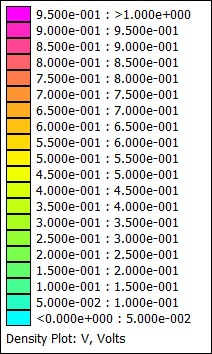
\includegraphics[width=\textwidth]{data/Skala}
		\caption{Skala}
		\label{fig:Skala}
	\end{subfigure}
	\begin{subfigure}[c]{0.38\textwidth}
		
\includegraphics[width=\textwidth]{data/KeineRandbedingungen}
		\caption{Direkte Berandung}
		\label{fig:kleinRand}
	\end{subfigure}
	\begin{subfigure}[c]{0.38\textwidth}
		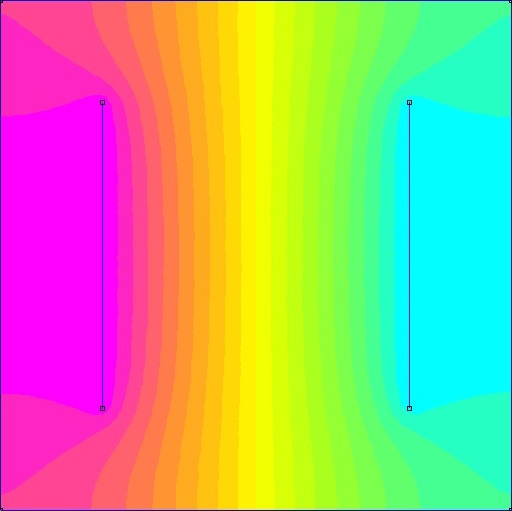
\includegraphics[width=\textwidth]{data/RandGross}
		\caption{Berandung durch Käfig}
		\label{fig:KäfigRand}
	\end{subfigure}
	\caption{Aufbau und Feldlinien des Kondensators}
\end{figure}

Vergleich man nun den Plot \ref{fig:kleinRand} mit \ref{fig:KäfigRand}, so wird eindeutig, dass die Feldlinien in Abbildung \ref{fig:kleinRand} senkrecht zu den beiden Flächen stehen. Berandet man den Kondensator durch einen Käfig, so werden auch die nicht senkrecht verlaufenden Feldlinien beachtet. In beiden Fällen entsteht ein homogenes Feld. Auch bei der Kapazität lassen sich unterschiedliche Werte ablesen. Während der Kondensator \ref{fig:kleinRand} eine Kapazität von \SI{2,6562}{\pico\coulomb} hat, liegt die Kapazität von Kondensator \ref{fig:KäfigRand} bei \SI{3,9773}{\pico\coulomb} \newpage
Zusätzlich soll verglichen werden, wie sich verschiedene Randbedingungen auf das entstehende elektrische Feld auswirken. Hierzu wurden dem Rand verschiedene Werte zugewiesen. Zunächst in Abbildung \ref{fig:0V} eine Spannung von \SI{0}{\volt}, dann in Abbildung \ref{fig:0,5V} \SI{0,5}{\volt} und schließlich eine Spannung von \SI{1}{\volt} in Abbildung \ref{fig:1V}. Es gilt die Selbe Skala, die in \ref{fig:Skala} zu sehen ist.

\begin{figure}[h]
	\begin{subfigure}[c]{0.32\textwidth}
		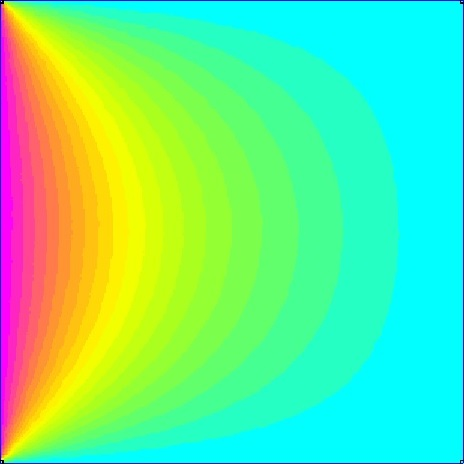
\includegraphics[width=\textwidth]{data/0VRandbedingung}
		\caption{Rand mit 0V Spannung}
		\label{fig:0V}
	\end{subfigure}
	\begin{subfigure}[c]{0.32\textwidth}
		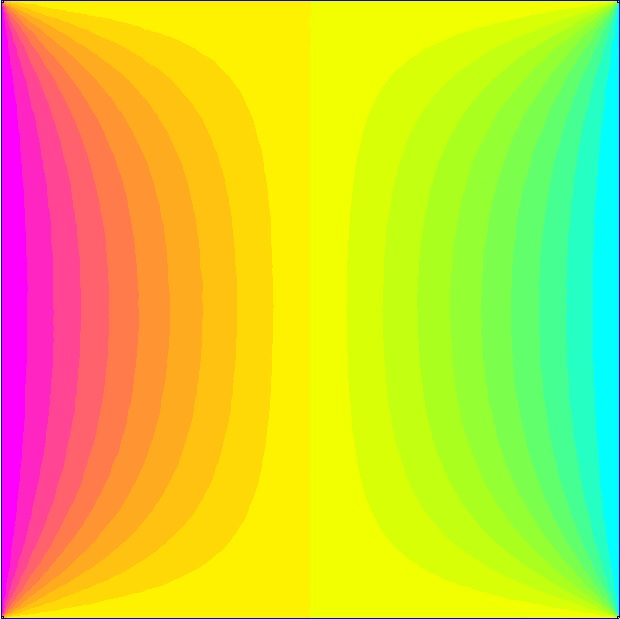
\includegraphics[width=\textwidth]{data/0,5VRandbedingung}
		\caption{Rand mit 0,5V Spannung}
		\label{fig:0,5V}
	\end{subfigure}
	\begin{subfigure}[c]{0.32\textwidth}
		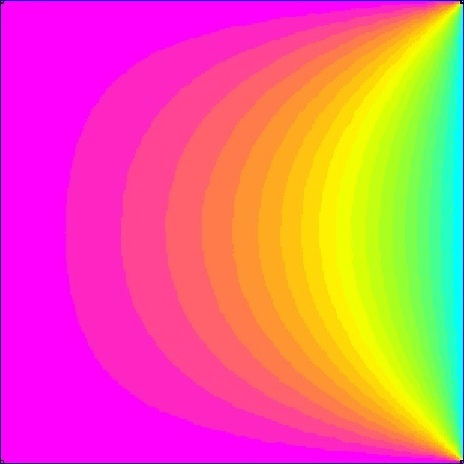
\includegraphics[width=\textwidth]{data/1VRandbedingung}
		\caption{Rand mit 1V Spannung}
		\label{fig:1V}
	\end{subfigure}
	\caption{Darstellung unterschiedlicher Randbedingungen}
\end{figure}

Da nun unterschiedliche Randbedingungen herrschen, entstehen auch Feldlinien zwischen den Kondensatorplatten und dem Rand. Es ergeben sich nicht nur unterschiedliche Feldlinien, sondern auch verschiedene Kapazitäten an den beiden Platten. 
\vspace*{1.5cm}

\begin{table}[h]
	\centering
	\begin{tabular}[h]{c|c c}
		Spannung am Rand & Kapazität linke Kondensatorplatte & Kapazität rechte Kondensatorplatte \\
		\hline
		\SI{0}{\volt} &  \SI{22,1405}{\pico\coulomb} & \SI{-0,5861}{\pico\coulomb} \\
		\SI{0,5}{\volt} & \SI{11,3633}{\pico\coulomb} & \SI{-11,3633}{\pico\coulomb} \\
		\SI{1}{\volt} &  \SI{0,5861}{\pico\coulomb} & \SI{-22,1405}{\pico\coulomb}
	\end{tabular}
\end{table}
\vspace*{1.5cm}
Die Feldlinien werden offensichtlich durch die anliegende Spannung am Rand beeinflusst und damit auch die Kapazität des Kondensators.
\\
\\
FEMM lässt sich nicht nur mit Hilfe von Octave starten, sondern es besteht auch die Möglichkeit eine OctaveFEMM Routine zu schreiben und damit ein Modell zu erstellen, sowie eine Simulation dieses Modells zu starten. In dem gegebenen Fall, soll eine Routine geschrieben werden, die zwei Parameter $a$ und $h$ entgegen nimmt, wobei $a$ die Kantenlänge und $h$ der Abstand der Platten ist. Aus diesen Informationen soll ein Kondensator erstellt und die berechnete Kapazität $C$ zurückgeliefert werden. Der Quellcode befindet sich im Anhang. \\ 
\newpage
Zunächst wird in Zeile 7 bis 9 FEMM geöffnet und definiert um welche Art von Problem es sich handelt. Zusätzlich werden einige Einstellungen getroffen, wie die Einheit der Variablen, die Tiefe des Modells und die Rechengenauigkeit. \\ 
In Zeile 10 bis 13 werden die verschiedenen Properties erzeugt, also die Randbedingungen (falls gewünscht), die Kondensatorplatten und das Dielektrikum. \\
Durch den Befehl in Zeile 16 wird daraufhin ein Rechteck, mit Hilfe der an die Methode übergebenen Parameter,  erstellt. Ein Blocklabel für das Dielektrikum wird in Zeile 19 erzeugt. Von Zeile 22 bis 38 werden nun die einzelnen Properties den richtigen Linien und Punkten zugewiesen.\\
Bevor die Simulation starten kann, muss das Projekt gespeichert werden. Danach wird die Analyse auf dieser Datei gestartet und die Lösung graphisch auf dem Bildschirm angezeigt.\\
Der zurückzuliefernde Parameter $C$ ergibt sich nun aus dem Ergebnis der Ladung geteilt durch die Spannung. Diese sind in einem liegenden Vektor mit zwei Spalten gespeichert. Die Ladung an zweiter und die Spannung an erster Stelle. 
	
	%%%%%%%%%%%%%%%%%%Fazit%%%%%%%%%%%%%%%%%%%%%%
	\chapter{Fazit}\label{sec:fazit}
%\addcontentsline{toc}{section}{Fazit}
Die erste Aufgabe ergab, dass sich die beiden Leiter des Koaxialkabels wie die Platten eines Plattenkondensators verhalten. Darüber hinaus ergibt sich, dass man durch Anfügen von weiteren Segmenten an die Schaltung eine Verkleinerung der Schwingfrequenz bewirkt.
Differentialgleichungen können häufig, wie sich in Aufgabe zwei zeigt, leichter im Frequenzbereich als im Zeitbereich gelöst werden. Die durch Lösen der Differentialgleichung analytisch berechneten Ergebnisse für Zeit- und Frequenzverhalten stimmen dabei mit der numerischen Simulation durch LTSpice überein.
Die Ergebnisse der dritten Aufgabe ergeben, dass sich die Feldlinien eines Kondensators in einem Simulationskäfig nicht nur senkrecht zu den Platten bewegen, sondern dass sich auch Randeffekte an den Enden der Kondensatorplatten ausbilden. Untersucht man unterschiedliche Randbedingungen zeigt sich, dass diese sowohl den Kapazitätswert des Kondensators, als auch die elektrischen Feldlinien beeinträchtigen. Die Wahl der Simulationsrandbedingungen kann also nicht willkürlich erfolgen.
	%%%%%%%%%%%%%%%%%%Anhang%%%%%%%%%%%%%%%%%%%%%
	\chapter{Anhang}\label{sec:anhang}
\lstset{ % Octave Settings
	language=Octave,
	extendedchars=true,
	basicstyle=\footnotesize,
	numbers=left,
	numberstyle=\tiny\color{gray},
	stepnumber=1,
	numbersep=10pt,
	showspaces=false,
	showstringspaces=false,
	tabsize=2,
	breaklines=true,
	frame=single,
	morecomment = [l][\itshape\color{blue}]{\%},
	captionpos=b,
	title=\lstname
}


\lstinputlisting{data/SIS.m}
\lstinputlisting{data/SkriptAg8_2.m}
\lstinputlisting{data/SkriptAg8_3d.m}



	%%%%%%%%%%%%%%%%%%%%%%%%%%%%%%%%%%%%%%%%%%%%%%%%%%%%%%%%%%%%%%%%%%%%%%%%%%%%%%%%%%%%%%%%%%%%%%%%%%
	
	%%%%%%%%%%%%%%%%%%%
	%Abbildungs- und Tabellenverzeichnis
	%%%%%%%%%%%%%%%%%%%
	\listoffigures % Abbildungsverzeichnis (captions in den Figuren werden als Referenz genommen)
	\listoftables % Verzeichnis der Tabellen (captions in den Tabellen werden als Referenz genommen)
	
	%%%%%%%%%%%%%%%%%%%
	%Literaturverzeichnis an dieser Stelle
	%%%%%%%%%%%%%%%%%%%
	
	
\end{document}
